\documentclass[spanish] {article}
\usepackage[T1]{fontenc}
\usepackage{selinput}
\usepackage{hyperref}
\usepackage{graphicx}
\SelectInputMappings{%
  aacute={á},
  eacute={é},
  iacute={í},
  oacute={ó},
  uacute={ú},
  ntilde={ñ},
  Euro={€}
}
\usepackage{babel}
\begin{document}
\title{Prueba de Oposición de Ayudantes 2da}
\author{
\includegraphics[width=32mm]{logo-fiuba}\\ \\ \Huge Facultad de Ingeniería\\ \\ \Large UBA \\ \\ \Large Gabriel La Torre}

\maketitle
\newpage
\section{Introducción}
A continuación se dará un enunciado de un ejericio de la guía de Ondas Mecánicas. Posteriormente se explicarán los supuestos a considerar antes de resolverlo, como por ejemplo, el conocimiento previo de los alumnos al momento de presentarles el ejercicio en cuestión.
Finalmente se resolverá el ejercicio con el agregado de algunas notas explicativas que den al lector una idea de la explicación que se dará en la clase.
\section{Enunciado}
La expresión de una cierta onda es $y = 10 sen [2 \pi (2x- 100 t)]$, donde x está en metros y t en 
segundos. Halle: 
\begin{enumerate}
\item La amplitud
\item La longitud de onda
\item La frecuencia
\item La velocidad de propagación de la onda. 
\item Trace un diagrama de la onda en el que se muestre la amplitud y la longitud de onda. 
\end{enumerate}

\section{Supuestos}
Al momento de presentarles este ejercicio, los alumnos ya tuvieron la introducción teórica a las ondas mecánicas. Saben identificar una función de onda, han sido informados de la definición de una onda y la diferencia entre ondas mecánicas y ondas electromagnéticas.
\section{Resolución}
Primero analizamos la fórmula
$$y = 10 sen [2 \pi (2x- 100 t)]$$
La forma de la función cumple con la forma de una función de onda
$$y = A sen (kx \pm \omega t + \varphi)]$$
De solo ver la forma podemos saber que la amplitud es 10 metros. Si bien no está explícito en la fórmula, al indicar, el enunciado, que $x$ está expresada en metros, es válido suponer que A también estará expresada en metros.

Si seguimos el análisis de la forma de la función y la modificamos un poco para que se parezca aún más a la expresada arriba
$$y = 10 sen  (4 \pi x- 200 \pi t)$$

Llegamos a la conclusión de que $4 \pi$ es el número de onda $k$ de la onda que estamos analizando. El alumnado, vio en la introducción teórica que 
$$ k = \frac{2\pi}{\lambda}$$
Por lo cual podemos proseguir a calcular la longitud de onda como
$$ \lambda = \frac{2\pi}{4\pi} = \frac{1}{2} = 0,5 metros$$ 
Finalmente $\lambda$ es igual a 0,5 metros. Es importante remarcar que la longitud de onda debe ser acompañada de su unidad correspondiente. En este momento, se le puede mencionar al alumno que esta longitud de onda está expresada en metros, pero que puede darse el caso en que se exprese en nanómetros, $\mathring{a}ngstr\ddot{o}m$ ($\mathring{A}$), etc.
Adicionalmente se puede inducir a pensar en esta onda como una cuerda que está siendo agitada y la distancia entre una cresta y la otra es de 0,5 metros, para que quede el concepto detrás de la longitud de onda.

Seguimos el análisis de la forma de la función de la onda y podemos apreciar que $ \omega = 200 \pi $. Los alumnos vieron en la clase teórica la relación $ \omega = 2 \pi f $
Por lo cual resulta trivial resolver
$$ f = \frac{200 \pi}{2 \pi} = 100 seg^{-1}$$
Nuevamente es importante aclarar que la frecuencia tiene una unidad asociada y que en este caso es $1/seg$.
Ahora que tenemos la frecuencia y la longitud de onda podemos hacer uso de la fórmula $v = \lambda \cdot f$ dada en la teórica para obtener la velocidad de propagación de la onda
$$v = 0,5m \cdot 100 \frac{1}{seg} = 0,005 \frac{m}{seg}$$

A continuación elegiremos un t determinado, en este caso t = 0 y graficaremos la ecuación de onda resultante $y=10 sen(4 \pi x)$

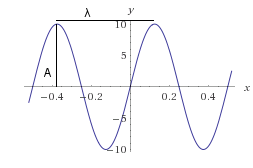
\includegraphics{plot2}

Acá podemos observar como la amplitud es el valor del máximo de la función de onda y la longitud de onda es la distancia en $x$ entre un período y otro de la onda, se puede observar en el gráfico por ejemplo en la distancia entre dos crestas sucesivas.

\section{Referencias}

\begin{itemize}
  \item \href{http://wiki.foros-fiuba.com.ar/_media/materias:62:guia_fisica_i_62.01.pdf}{Guía de Ejercicios Física I 62.01}.
\end{itemize}
\end{document}
